\section{BAYESIAN NETWORKS}
\label{sec:bns}

Bayesian networks are a general way to describe the dependencies
between the components of an $n$\nobreakdash-dimensional discrete data
vector $X=(X_{1},\ldots,X_{n})$ in which the component $X_{i}$ may
take any of the discrete values in a set $\{1,\ldots,r_{i}\}$.
Despite denoting the values with small integers, the model will treat
the components of $X$ as categorical variables.


\subsection{Likelihood}
\label{ssec:likelihood}

A Bayesian network $B=(G,\theta)$ defines a probability distribution for
$X$. The component $G$ defines the structure of the model as a
directed acyclic graph (DAG) that has exactly one node for each component of
$X$. The structure $G=(G_{1},\ldots,G_{n})$ defines for each
variable/node $X_{i}$ its (possibly empty) parent set $G_{i}$, i.e.,
the nodes from which there are a directed edges to the variable
$X_{i}$.

Given a realization $x$ of $X$, we denote the sub\nobreakdash-vector
of $x$ that consists of the values of the parents of $X_{i}$ in $x$ by
$G_{i}(x)$. It is customary to enumerate all the possible
sub\nobreakdash-vectors $G_{i}(x)$ from $1$ to $q_{i}=\prod_{h\in
  G_{i}}r_{h}.$ In case $G_{i}$ is empty, we define $q_{i}=1$ and
$P(G_{i}(x)=1)=1$ for all vectors $x$.

For each variable $X_{i}$ there is a $q_{i}\times r_{i}$ table
$\theta_{i}$ of parameters whose $k^{\textnormal{th}}$ column
on the $j^{\textnormal{th}}$ row $\theta_{ij}$ defines the conditional
probability $P(X_{i}=k\mid G_{i}(X)=j;\theta)=\theta_{ijk}$.  With
structure $G$ and parameters $\theta$, we can now express the
likelihood function of the model as
\begin{equation}
P(x|G,\theta)=\prod_{i=1}^{n}P(x_{i}\mid
G_{i}(x);\theta_{i})=\prod_{i=1}^{n}\theta_{iG_{i}(x)x_{i}}.
\end{equation}



\subsection{Bayesian Structure Learning}

Score-based Bayesian learning of Bayesian network structures evaluates the goodness of different structures $G$ using their
posterior probability $P(G|D,\alpha)$, where $\alpha$ denotes the
hyperparameters for the model parameters $\theta$, and the $D$ is a
collection of $N$ $n$\nobreakdash-dimensional i.i.d. data vectors
collected to a $N\times n$ design matrix. We use the notation $D_i$ to
denote the $i^\text{th}$ column of the data matrix and notation $D_V$ to denote
the columns that correspond to the variable subset $V$. We also write
$D_{i,G_i}$ for $D_{\{i\}\cup G_i}$ and denote the entries of the
column $i$ on the rows on which the parents $G_i$ contain the value
configuration number by $D_{i,G_i=j}$, $j\in\{1,\ldots,q_i\}$.

It is common to assume the uniform prior for structures, in which case
the objective function for structure learning is reduced to the
marginal likelihood $P(D|G,\alpha)$.  If the model parameters
$\theta_{ij}$ are further assumed to be independently Dirichlet
distributed only depending on $i$ and $G_{i}$ and the data $D$ is
assumed to have no missing values, the marginal likelihood can be
decomposed as
\begin{eqnarray}
\label{eqn:bayesmix}
\lefteqn{P(D|G,\alpha)}\nonumber\\
&&=\prod_{i=1}^{n}\prod_{j=1}^{q_i}P(D_{i,G_i=j};\alpha)\nonumber\\
&&=\prod_{i=1}^{n}\prod_{j=1}^{q_i}\int P(D_{i,G_i=j}|\theta_{ij})P(\theta_{ij};\alpha) d\theta_{ij}.
\end{eqnarray}
In coding terms this means that each data column $D_i$ is first
partitioned based on the values in columns $G_i$, and each part is
then coded using a Bayesian mixture that can be expressed in a closed
form~\cite{Bunt91, Heck95}. 

\begin{figure}
\centering
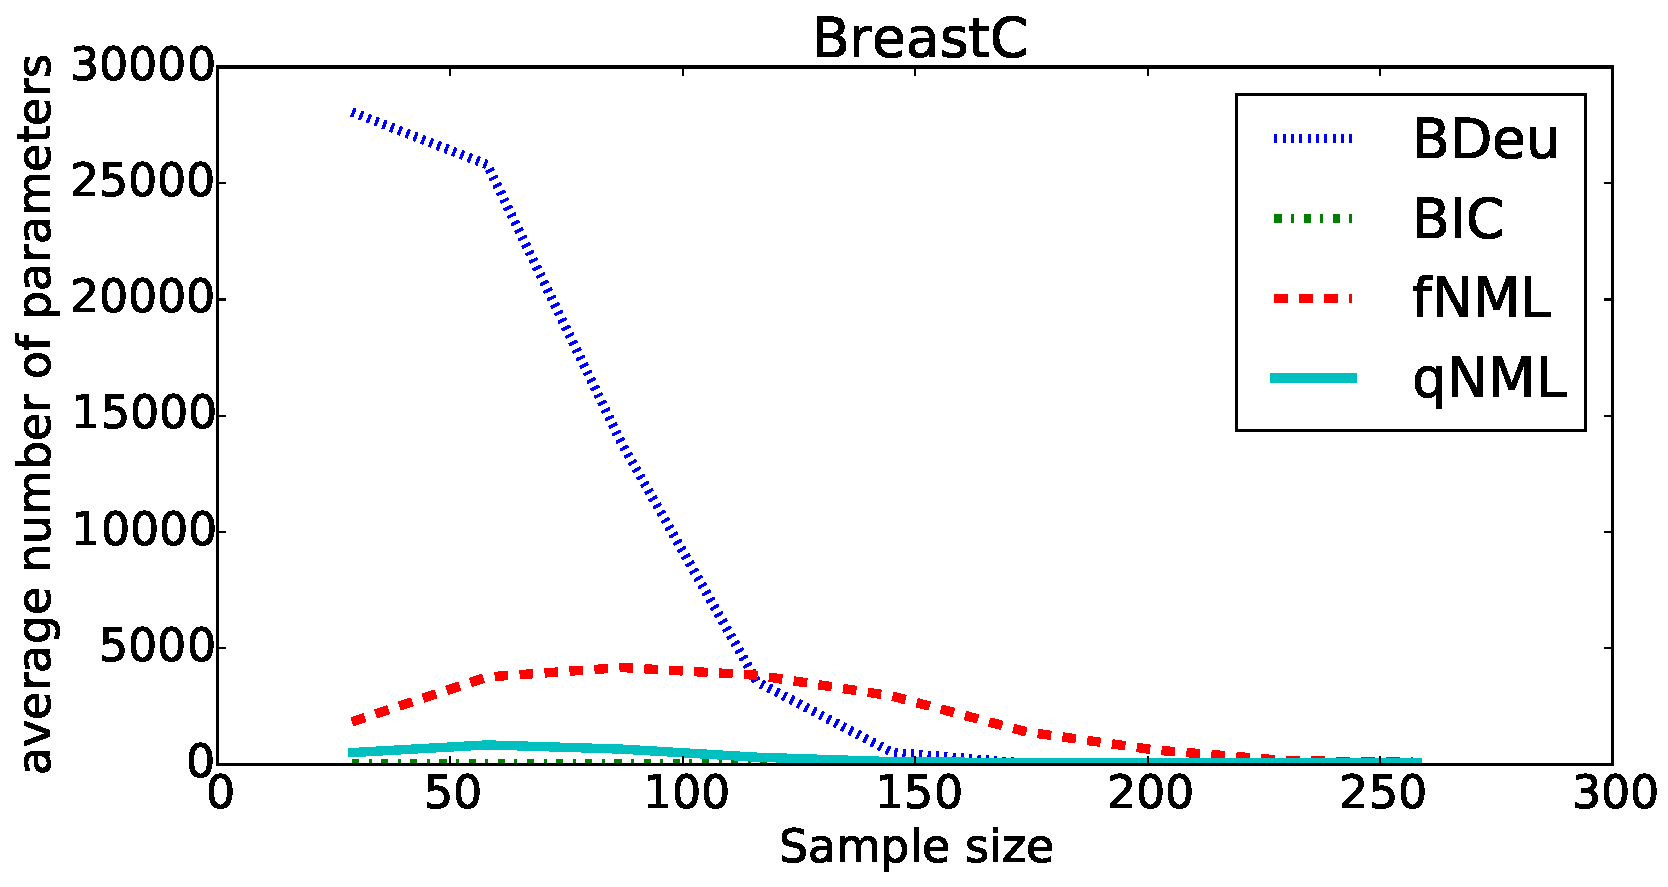
\includegraphics[width=8cm,height=5cm]{qNML_images/breast_cancer_npmean.pdf}
\caption{Number of parameters in a breast cancer model as a function
  of sample size for different model selection criteria.}
\label{fig:bcnpmean}
\end{figure}


\subsection {Problems, Solutions and Problems}

Finding satisfactory Dirichlet hyperparameters for the Bayesian
mixture above has, however, turned out to be problematic. Early on,
one of the desiderata for a good model selection criterion was that it
is score equivalent, i.e., it would yield equal scores for
essentially equivalent models~\cite{Verm90}.  For example, the score
for the structure $X_1\rightarrow X_2$ should be the same as the score
for the model $X_2 \rightarrow X_1$ since they both correspond to the
hypothesis that variables $X_1$ and $X_2$ are statistically dependent
on each other.  It can be shown~\cite{Heck95} that to achieve this,
not all the hyperparameters $\alpha$ are possible and for practical
reasons Buntine~\cite{Bunt91} suggested a so-called BDeu score with
just one hyperparameter $\alpha\in R_{++}$ so that
$\theta_{ij\cdot}\sim Dir(\frac{\alpha}{q_i
  r_i},\ldots,\frac{\alpha}{q_i r_i})$.  However, it soon turned out
that the BDeu score was very sensitive to the selection of this
hyperparameter~\cite{cosco.uai07} and that for small sample sizes this
method detects spurious correlations~\cite{Steck08} leading to models
with suspiciously many parameters.

Recently, Suzuki~\cite{Suzuki2017} discussed the theoretical
properties of the BDeu score and showed that in certain settings BDeu
has tendency to add more and more parent variables for a child node
even though the empirical conditional entropy of the child given the
parents has already reached zero. In more detail, assume that in our
data $D$, the values of $X_i$ are completely determined by variables
in set $Z$, so that the empirical entropy $H_N(X_i | Z) = 0$. Now, if we can further
find one or more variables, denoted by $Y$, whose values are
determined completely by the variables in $Z$, then BDeu will prefer
the set $Z\cup Y$ over $Z$ alone as the parents of $X_i$. Suzuki
argues that this kind of behaviour violates \textit{regularity} in model
selection as the more complex model is preferred over a simpler one
even though it does not fit the data any better. The phenomenon seems
to stem from the way the hyperparameters for the Dirichlet
distribution are chosen in BDeu as using Jeffreys' prior,
$\theta_{ijk}\sim Dir(\frac{1}{2},\ldots,\frac{1}{2})$, does not suffer
from this anomaly. However, using Jeffreys' prior causes marginal
likelihood score not to be score equivalent. In Section \ref{sec:regularity}, we will give the formal definition of regularity and state that qNML is regular. In addition, we provide a proof of regularity for fNML criterion, which has not appeared in the literature before. The detailed proofs can be found in Appendix B in the Supplementary Material.     

A natural solution to avoid parameter sensitivity of BDeu would be to
use a normalized maximum likelihood (NML)
criterion~\cite{Shta87,Riss96a}, i.e., to find the structure $G$ that
maximizes
\begin{equation}
P_{NML}(D;G)=\frac{P(D|\hat\theta(D;G))}{\sum_{D'}{P(D'|\hat\theta(D';G))}},
\end{equation}
where $\hat\theta$ denotes the (easy to find) maximum likelihood
parameters and the sum in the denominator goes over all the possible
$N\times n$ data matrices. This information-theoretic NML criterion
can be justified from the minimum description length point of view,
\cite{Riss78,Grun07}. It has been shown to be robust with respect to
different data generating mechanisms where a good choice of prior
is challenging, see~\cite{eggeling2014robust,maatta16}. While it is
easy to see that the NML criterion satisfies the requirement of giving
equal scores to equal structures, the normalizing constant renders the
computation infeasible.

Consequently, Silander et al.~\cite{cosco.pgm08a}
suggested solving the BDeu parameter sensitivity problem by using the
NML-code for the column partitions, i.e., changing the Bayesian mixture
in equation~(\ref{eqn:bayesmix}) to
\begin{equation}
P^1_{NML}(D_{i,G_i=j};G)=\frac{P(D|\hat\theta(D_{i,G_i=j};G))}{\sum_{D'}{P(D'|\hat\theta(D';G))}},
\end{equation}
where $D'\in{\{1,\ldots,r_i\}}^{|D_{i,G_i=j}|}$.  The logarithm of the
denominator is often called a regret, since it indicates the extra
code length needed compared to the code length obtained using the (a
priori unknown) maximum likelihood parameters. The regret for
$P^1_{NML}$ depends only on the length $N$ of the categorical data
vector with $r$ different categorical values,
\begin{equation}
reg(N,r)=\log \sum_{D\in \{1,\ldots,r\}^N} P(D|\hat\theta(D)).
\end{equation}
While the naive
computation of the regret is still prohibitive, Silander et al.\
approximate it efficiently using a so-called Szpankowski
approximation~\cite{cosco.aistat03}:
\begin{eqnarray}
\label{eqn:szp1}
\lefteqn{reg(N,r) \approx \frac{\sqrt{2} r \Gamma{\left(\frac{r}{2} \right)}}
                               {3 \sqrt{N} \Gamma{\left(\frac{r-1}{2}  \right)}}} \\
&&+ \left(\frac{r-1}{2}\right) \log{\left (\frac{N}{2} \right )}
- \log \Gamma{\left(\frac{r}{2} \right)} + \frac{1}{2} \log{\left (\pi \right )}\nonumber\\
&&- \frac{r^{2} \Gamma^{2}{\left(\frac{r }{2} \right)}}
         {9N \Gamma^{2}{\left(\frac{r-1}{2}\right)}}
+ \frac{2r^3-3r^2-2r+3}{36N}\nonumber.
\end{eqnarray}

However, equation (\ref{eqn:szp1}) is derived only for the case
where $r$ is constant and $N$ grows. While with
fNML it is typical that $N$ is large compared to $r$, an
approximation for all ranges of $N$ and $r$ derived by
Szpankowski and Weinberger~\cite{Szpankowski2012} can also be used:
\begin{eqnarray}
\label{eqn:szp2}
    reg(N, r) & \approx & N\left(\log{\alpha} + (\alpha + 2) \log{C_\alpha}
                - \frac{1}{C_\alpha}\right)\nonumber \\
    && - \frac{1}{2} \log{\left(C_\alpha + \frac{2}{\alpha}\right)},
\end{eqnarray}
where $\alpha = \frac{r}{N}$ and
%\begin{equation}
    $C_\alpha = \frac{1}{2} + \frac{1}{2} \sqrt{1 + \frac{4}{\alpha}}$.
%\end{equation}
These approximations are compared in Table \ref{tbl:regrets} to the
exact regret for various values of $N$ and $r$.  For a constant $N$,
equation (\ref{eqn:szp1}) provides a progressively worse approximation
as $r$ grows. Equation (\ref{eqn:szp2}) on the other hand is a good
approximation of the regret regardless of the ratio of $N$ and $r$.
In our experiments, we will use this approximation for 
implementation of the qNML criterion.


fNML solves the parameter sensitivity problem and yields predictive
models superior to BDeu.  However, the criterion does not satisfy the
property of giving the same score for models that correspond to the
same dependence statements. The score equivalence is usually viewed desirable when DAGs are considered only as models for conditional independence, without any causal interpretation. Furthermore, the learned structures are
often rather complex (see Figure~\ref{fig:bcnpmean}) which also
hampers their interpretation. The quest for a model selection
criterion that would yield more parsimonious, easier to interpret, but
still predictive Bayesian networks structures is one of the main
motivations for this work.


\begin{table}
\caption{Regret values for various values of $N$ and $r$.}
\label{tbl:regrets}
\begin{center}
\begin{tabular}{crrrr}
N & r & eq. (\ref{eqn:szp1}) & eq. (\ref{eqn:szp2}) & exact \\
\midrule
\multirow{4}{*}{50} & 10 & 13.24 & 13.26 & 13.24 \\
& 100 & 62.00 & 60.01 & 60.00 \\
& 1000 & 491.63 & 153.28 & 153.28 \\
& 10000 & 25635.15 & 265.28 & 265.28 \\
\midrule
\multirow{4}{*}{500} & 10 & 22.67 & 22.69 & 22.67 \\
& 100 & 144.10 & 144.03 & 144.03 \\
& 1000 & 624.35 & 603.93 & 603.93 \\
& 10000 & 4927.24 & 1533.38 & 1533.38 \\
\midrule
\multirow{4}{*}{5000} & 10 & 32.74 & 32.76 & 32.74 \\
& 100 & 247.97 & 247.97 & 247.97 \\
& 1000 & 1452.51 & 1451.78 & 1451.78 \\
& 10000 & 6247.83 & 6043.16 & 6043.16 \\
\bottomrule
\end{tabular}
\end{center}
\end{table}
